% 请确保文件编码为utf-8,使用XeLaTex进行编译,或者通过overleaf进行编译

\documentclass[answers]{exam}  % 使用此行带有作答模块
% \documentclass{exam} % 使用此行只显示题目

\usepackage{xeCJK}
\usepackage{zhnumber}
\usepackage{graphicx}
\usepackage{hyperref}
\usepackage{amsmath}
\usepackage{booktabs}
\usepackage{enumerate}

\pagestyle{headandfoot}
\firstpageheadrule
\firstpageheader{南京大学}{数字信号处理}{习题集三}
\runningheader{南京大学}
{数字信号处理}
{习题集三}
\runningheadrule
\firstpagefooter{}{第\thepage\ 页(共\numpages 页)}{}
\runningfooter{}{第\thepage\ 页(共\numpages 页)}{}

% no box for solutions
% \unframedsolutions

\setlength\linefillheight{.5in}

% \renewcommand{\solutiontitle}{\noindent\textbf{答:}}
\renewcommand{\solutiontitle}{\noindent\textbf{解:}\par\noindent}

\renewcommand{\thequestion}{\zhnum{question}}
\renewcommand{\questionlabel}{\thequestion .}
\renewcommand{\thepartno}{\arabic{partno}}
\renewcommand{\partlabel}{\thepartno .}

\begin{document}
\Large
\centering{姓名:周韧哲 \qquad 学号:181220076 \qquad 邮箱:zhourz@smail.nju.edu.cn}
\begin{questions}
	
	

% question_1
\question 求图~\ref{Figure:question_1}所示各信号的拉普拉斯变换。
\begin{figure}[!h]
	\centering
	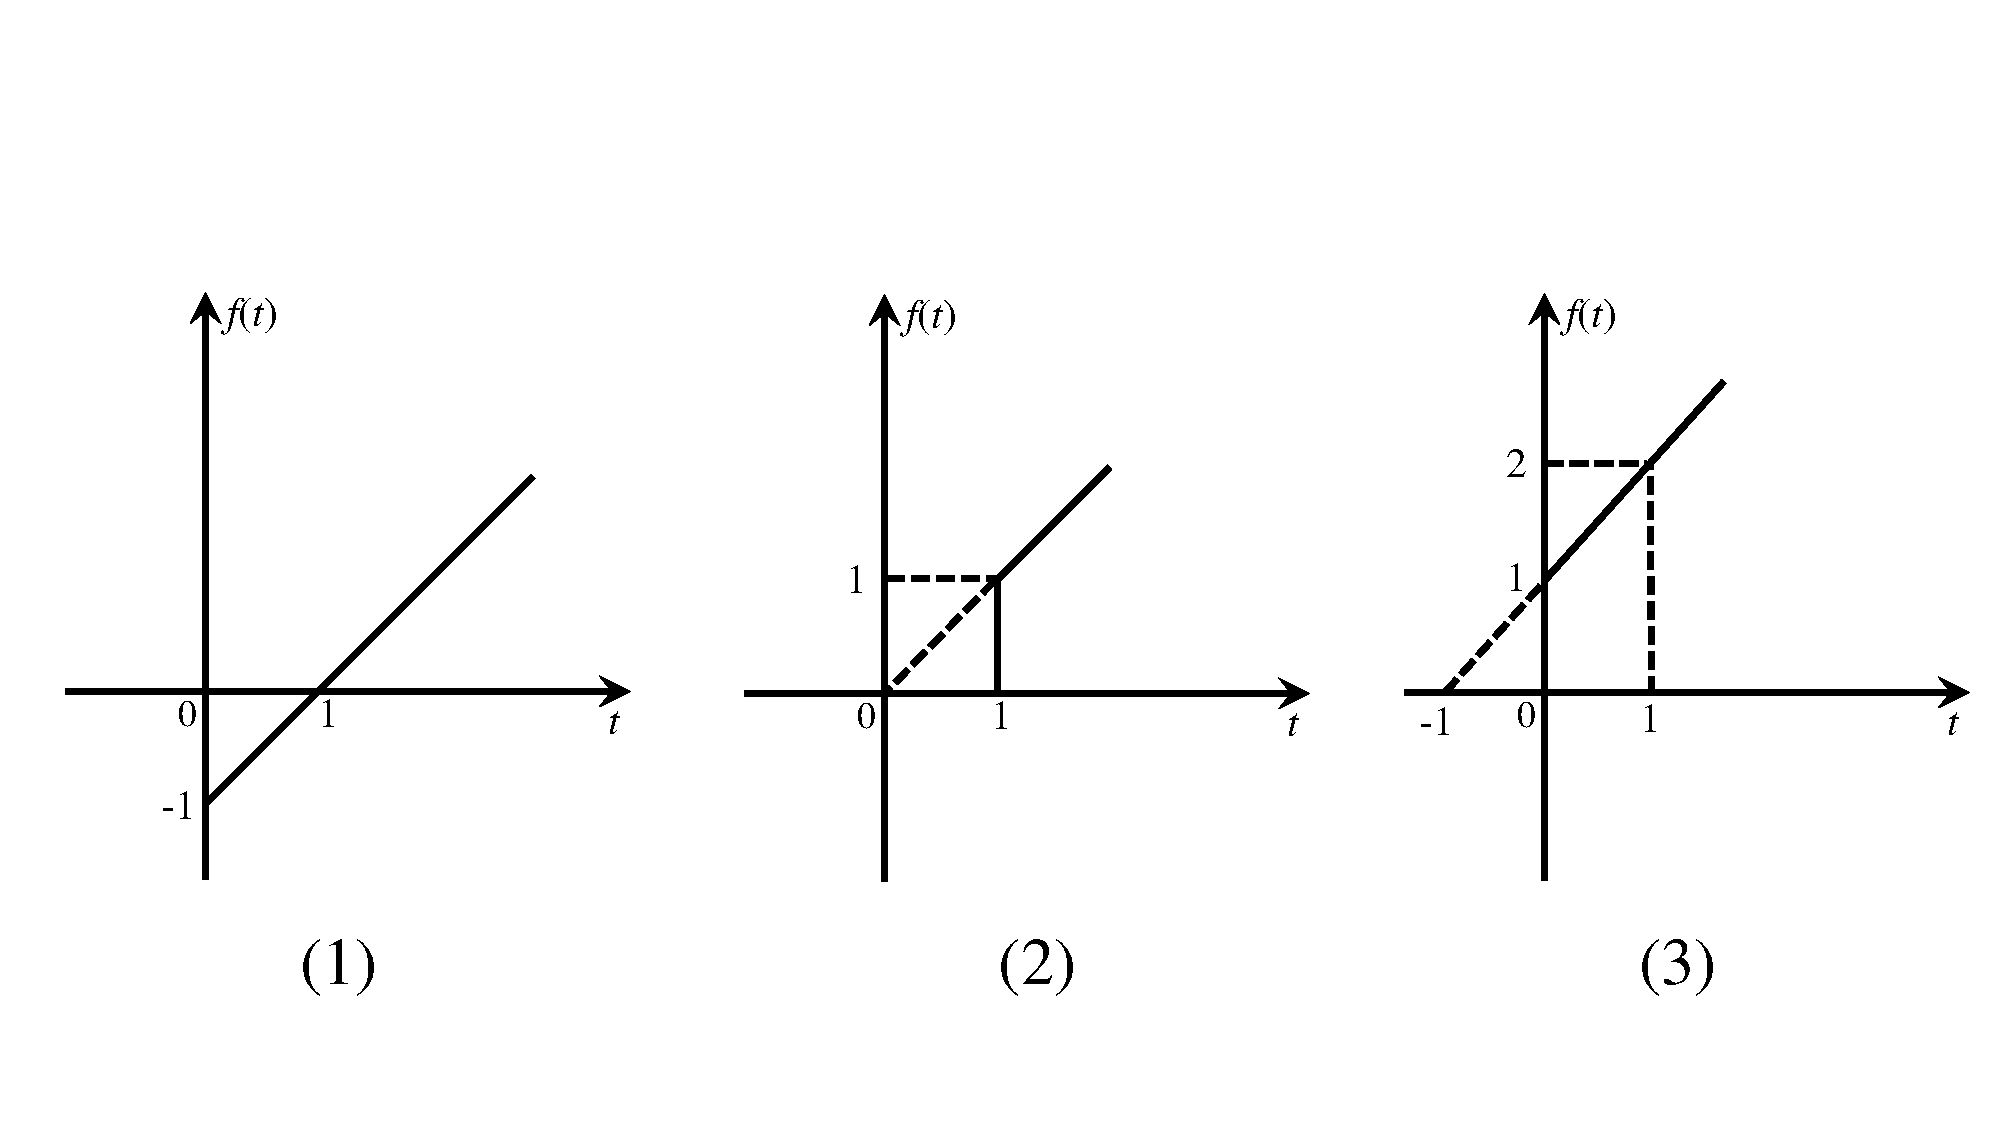
\includegraphics[width=\linewidth]{pics/question_1.pdf}
	\label{Figure:question_1}
	\caption{第一题图}
\end{figure}
\begin{solution}
\begin{enumerate}[(1)]
	\item 易知$x(t)=t-1,t\geq0$,从而\begin{align*}
		\mathcal{L}[x(t)]&=\int_{0_-}^{\infty}(t-1)e^{-st}dt\\
		&=-\frac{1}{s}\int_{0_-}^{\infty}(t-1)de^{-st}\\
		&=-\frac{1}{s}[(t-1)e^{-st}\big|_{0_-}^{\infty}-\int_{0_-}^{\infty}e^{-st}d(t-1)]\\
		&=-\frac{1}{s}+\frac{1}{s^2}
	\end{align*}
    \item 易知$x(t)=t,t>1$,从而\begin{align*}
    	\mathcal{L}[x(t)]&=\int_{1}^{\infty}te^{-st}dt\\
    	&=-\frac{1}{s}\int_{1}^{\infty}tde^{-st}\\
    	&=-\frac{1}{s}[te^{-st}\big|_{1}^{\infty}-\int_{1}^{\infty}e^{-st}dt]\\
    	&=(\frac{1}{s}+\frac{1}{s^2})e^{-s}
    \end{align*}
    \item 易知$x(t)=t+1,t\geq0$,从而\begin{align*}
    	\mathcal{L}[x(t)]&=\int_{0_-}^{\infty}(t+1)e^{-st}dt\\
    	&=-\frac{1}{s}\int_{0_-}^{\infty}(t+1)de^{-st}\\
    	&=-\frac{1}{s}[(t+1)e^{-st}\big|_{0_-}^{\infty}-\int_{0_-}^{\infty}e^{-st}d(t+1)]\\
    	&=\frac{1}{s}+\frac{1}{s^2}
    \end{align*}
\end{enumerate}
\end{solution}

% question_2
\question 求图~\ref{Figure:question_2}所示信号$f(t)$的拉普拉斯变化$F(s)$.
\begin{figure}[!h]
	\centering
	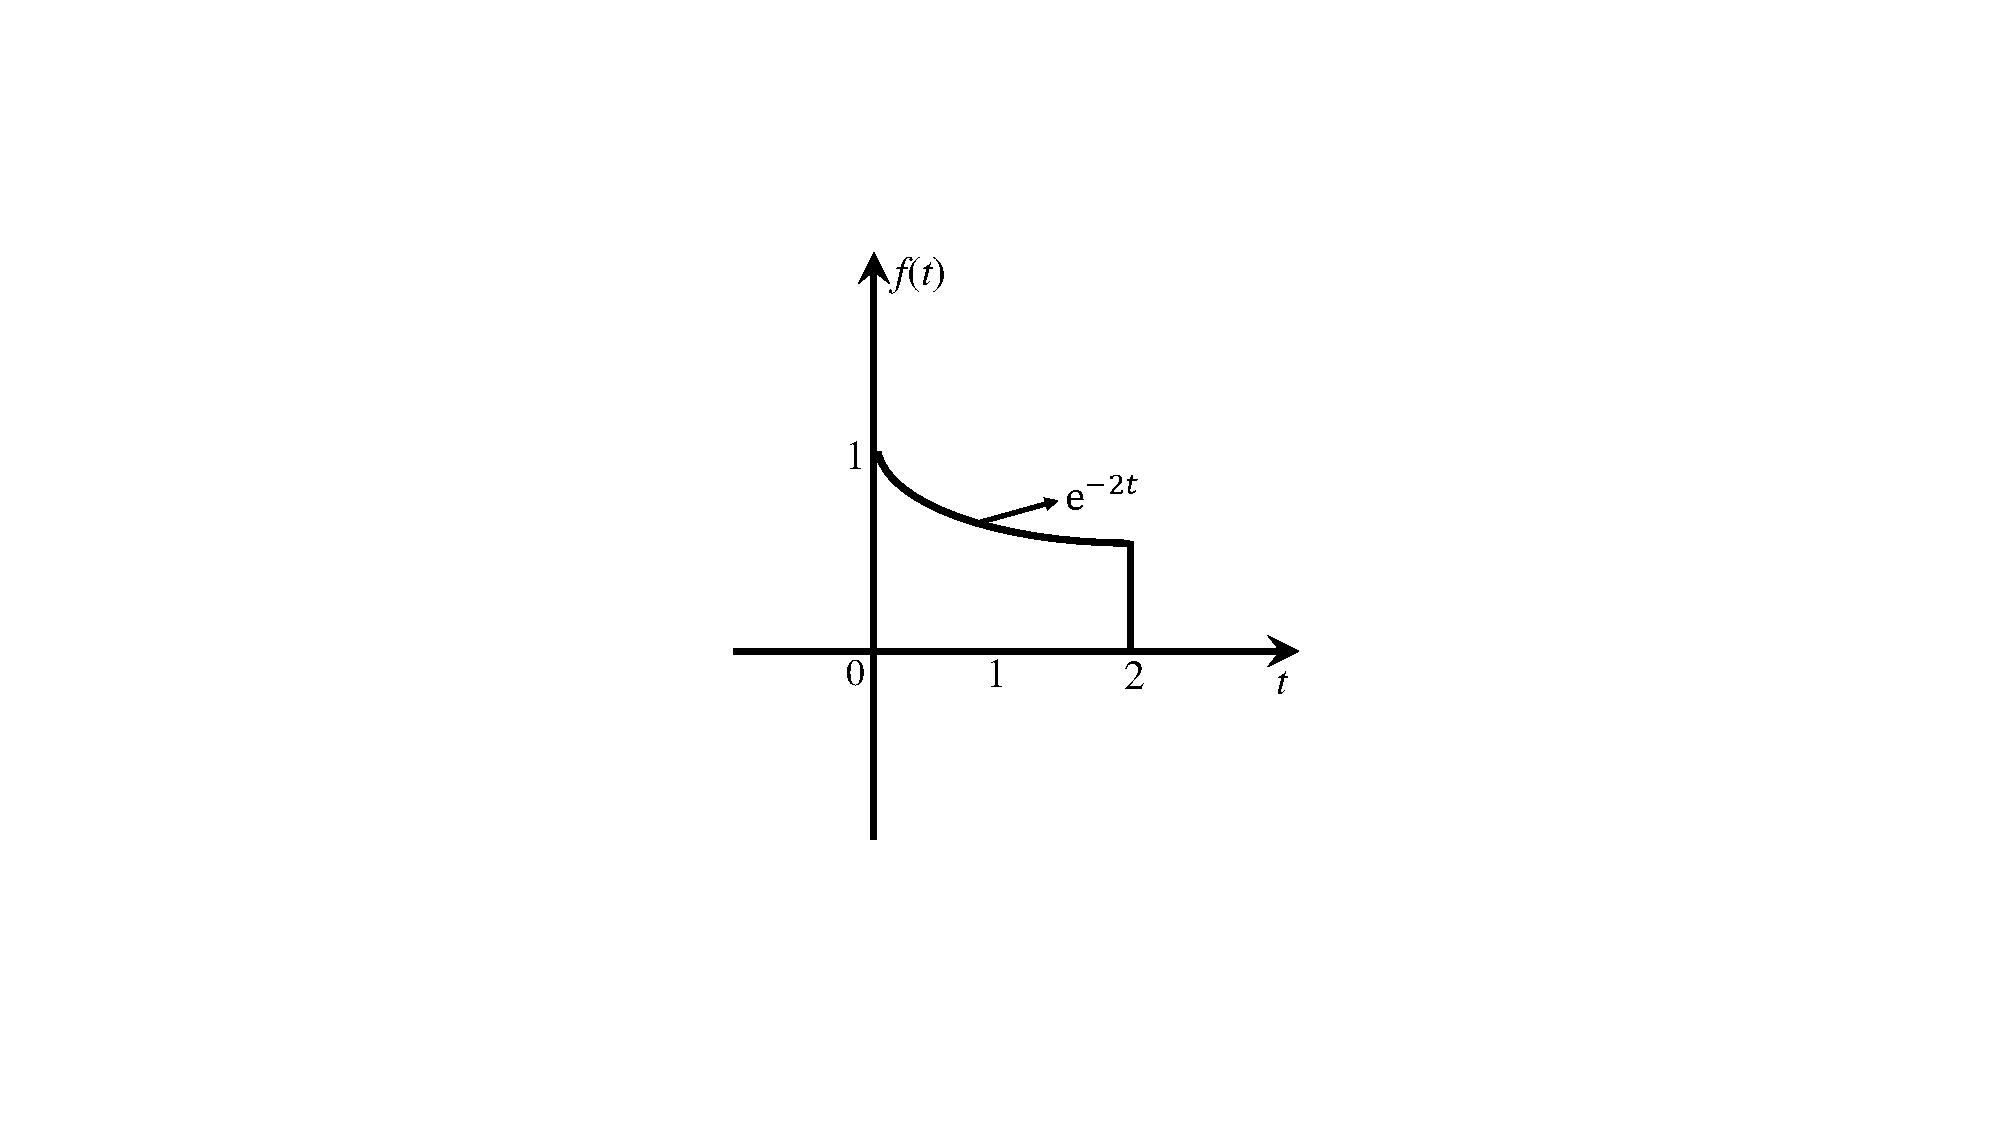
\includegraphics[width=0.3\linewidth]{pics/question_2.pdf}
	\label{Figure:question_2}
	\caption{第二题图}
\end{figure}
\begin{solution}
	易知$x(t)=e^{-2t},0\leq t\leq 2$,所以\begin{align*}
		F(s)&=\int_{0_-}^{\infty}e^{-2t}e^{-st}dt\\
		&=\int_{0_-}^{2}e^{-(2+s)t}dt\\
		&=\frac{1}{2+s}(1-e^{-2(s+2)})
	\end{align*}
\end{solution}

% question_3
\question 某系统函数$H(s)=\frac{1}{s^2+3s+1}$,若输入$x(t)=u(t)$,求出系统的零状态响应$y(t)$。
\begin{solution}
激励信号的拉普拉斯变换为$X(s)=\frac{1}{s},Re(s)>0$,由系统函数的定义易知,零状态响应的拉氏变换为$$Y_{zs}(s)=H(s)X(s)=\frac{1}{s^3+3s^2+s}=\frac{1}{s(s+\frac{3+\sqrt{5}}{2})(s+\frac{3-\sqrt{5}}{2})}$$使用部分分式展开法,得到$$Y_{zs}(s)=\frac{1}{s}+\frac{\frac{2}{5+3\sqrt{5}}}{s+\frac{3+\sqrt{5}}{2}}+\frac{\frac{2}{5-3\sqrt{5}}}{s+\frac{3-\sqrt{5}}{2}}$$
对上式进行拉式反变换得到$$y(t)=u(t)+\frac{2}{5+3\sqrt{5}}e^{-\frac{3+\sqrt{5}}{2}t}u(t)+\frac{2}{5-3\sqrt{5}}e^{-\frac{3-\sqrt{5}}{2}t}u(t)$$
\end{solution}

\begin{figure}[!h]
	\centering
	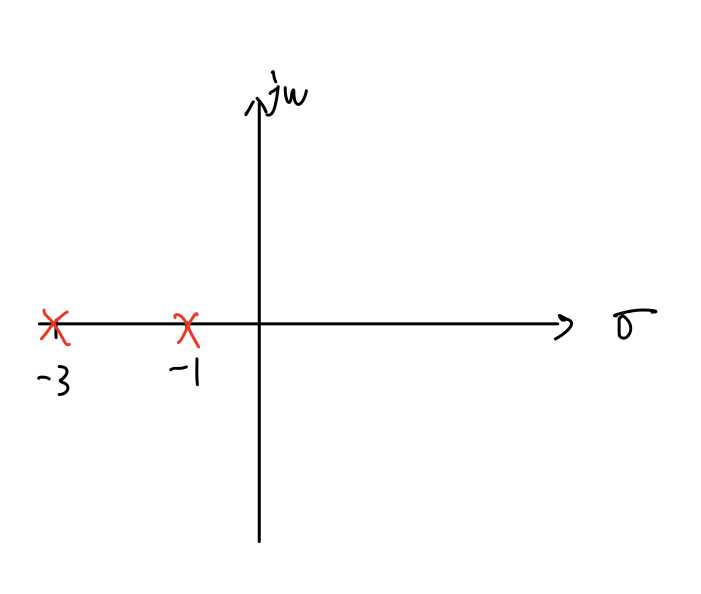
\includegraphics[width=0.5\linewidth]{pics/1.png}
	\label{Figure:q4}
	\caption{q4-零极点图}
\end{figure}
% question_4
\question 已知某线性时不变系统的微分方程为$\frac{\mathrm{d}^2y(t)}{\mathrm{d}t^2}+4\frac{\mathrm{d}y(t)}{\mathrm{d}t}+3y(t)=2x(t)$。
\begin{enumerate}[(1)]
\item 求该系统的系统函数,画出零极点图并判断该系统是否稳定。
\item 求该系统的冲激响应.
\end{enumerate}
\begin{solution}
\begin{enumerate}[(1)]
	\item 对微分方程两边进行LT,$(s^2+4s+3)Y_{zs}(s)=2X(s)$,从而系统函数$H(s)=\frac{Y_{zs}(s)}{X(s)}=\frac{2}{s^2+4s+3}=\frac{2}{(s+1)(s+3)}$。零极点图为\ref{Figure:q4}。极点都位于s左半平面,所以该系统稳定。
	\item $H(s)=\frac{1}{s+1}-\frac{1}{s+3}$,进行拉氏反变换,得到系统的冲激响应为$h(t)=(e^{-t}-e^{-3t})u(t)$。
\end{enumerate}
\end{solution}

% question_5
\question 求下列函数的拉普拉斯变换。
\begin{enumerate}[(1)]
\item $f(t)=\left\{\begin{matrix}
\sin(\omega t) & \text{当}\left(0<t<\frac{T}{2} \right )\\ 
 0& t\text{为其他值}
\end{matrix}\right.$

$T=\frac{2\pi}{\omega}$
\item $f(t)=\sin(\omega t+\phi)$
\end{enumerate}
\begin{solution}
\begin{enumerate}[(1)]
	\item 易得\begin{align*}
		f(t)&=\sin(wt)(u(t)-u(t-\frac{T}{2}))\\&=\sin(wt)u(t)-\sin(wt)u(t-\frac{T}{2})\\
		&=\sin(wt)u(t)+\sin(wt-\pi)u(t-\frac{T}{2})\\
		&=\sin(wt)u(t)+\sin(w(t-\frac{T}{2}))u(t-\frac{T}{2})
	\end{align*}
    所以由时移特性得\begin{align*}
    	\mathcal{L}[f(t)]&=\mathcal{L}[\sin(wt)u(t)]+\mathcal{L}[\sin(w(t-\frac{T}{2}))u(t-\frac{T}{2})]\\
    	&=\frac{w}{s^2+w^2}+\frac{w}{s^2+w^2}e^{-\frac{sT}{2}}\\
    	&=\frac{w}{s^2+w^2}(1+e^{-\frac{sT}{2}})
    \end{align*}
    \item 易得\begin{align*}
    	\mathcal{L}[f(t)]&=\mathcal{L}[\sin(wt+\phi)]\\
    	&=\mathcal{L}[\sin(wt)\cos\phi]+\mathcal{L}[\cos(wt)\sin\phi]\\
    	&=\frac{w}{s^2+w^2}\cos\phi+\frac{s}{s^2+w^2}\sin\phi\\
    	&=\frac{w\cos\phi+s\sin\phi}{s^2+w^2}
    \end{align*}
\end{enumerate}
\end{solution}

% question_6
\question 求下列函数的拉普拉斯变换。
\begin{enumerate}[(1)]
\item $f(t)=\mathrm{e}^{-t}u(t-2)$
\item $f(t)=\mathrm{e}^{-(t-2)}u(t-2)$
\item $f(t)=\mathrm{e}^{-(t-2)}u(t)$
\item $f(t)=\sin(2t)\cdot u(t-1)$
\item $f(t)=(t-1)[u(t-1)-u(t-2)]$
\end{enumerate}
\begin{solution}
\begin{enumerate}[(1)]
	\item \begin{align*}
		\mathcal{L}[f(t)]&=\mathcal{L}[e^{-2}e^{-(t-2)}u(t-2)]\\
		&=e^{-2}\int_{0_-}^{\infty}e^{-(t-2)}u(t-2)e^{-st}dt\\
		&=\int_{2}^{\infty}e^{-t-st}dt\\
		&=\frac{1}{1+s}e^{-2(1+s)}
	\end{align*}
    \item $$\mathcal{L}[f(t)]=e^2\mathcal{L}[e^{-t}u(t-2)]=\frac{1}{1+s}e^{-2s}$$
    \item $$\mathcal{L}[f(t)]=e^2\mathcal{L}[e^{-t}u(t)]=\frac{1}{1+s}e^{2}$$
    \item 由$f(t)=\sin(2(t-1)+2)u(t-1)=\sin(2(t-1))\cos2u(t-1)+\cos(2(t-1))\sin2u(t-1)$易得:\begin{align*}
    	\mathcal{L}[f(t)]&=\cos2\mathcal{L}[\sin(2(t-1))u(t-1)]+\sin2\mathcal{L}[\cos(2(t-1))u(t-1)]\\
    	&=\frac{2\cos2}{s^2+4}e^{-s}+\frac{s\sin2}{s^2+4}e^{-s}\\
    	&=\frac{2\cos2+s\sin2}{s^2+4}e^{-s}
    \end{align*}
    \item \begin{align*}
    	\mathcal{L}[f(t)]&=\mathcal{L}[(t-1)u(t-1)]-\mathcal{L}[(t-2)u(t-2)]-\mathcal{L}[u(t-2)]\\&=\frac{1}{s^2}e^{-s}-\frac{1}{s^2}e^{-2s}-\frac{1}{s}e^{-2s}\\
    	&=\frac{e^{-s}}{s^2}(1-(1+s)e^{-s})
    \end{align*}
\end{enumerate}
\end{solution}

% question_7
\question 求下列函数的拉普拉斯逆变换。
\begin{enumerate}[(1)]
\item $\frac{1}{s+1}$
\item $\frac{4}{2s+3}$
\item $\frac{4}{s(2s+3)}$
\item $\frac{3}{(s+4)(s+2)}$
\item $\frac{1}{s^2-3s+2}$
\item $\frac{1}{(s^2+3)^2}$
\end{enumerate}
\begin{solution}
\begin{enumerate}[(1)]
	\item $$\mathcal{L}^{-1}[\frac{1}{1+s}]=e^{-t}u(t)$$
	\item $$\mathcal{L}^{-1}[\frac{4}{2s+3}]=\mathcal{L}^{-1}[\frac{2}{s+\frac{3}{2}}]=2e^{-\frac{3}{2}t}u(t)$$
	\item 由部分分式展开得到$\frac{4}{s(2s+3)}=\frac{\frac{4}{3}}{s}-\frac{\frac{4}{3}}{s+\frac{3}{2}}$,所以$$\mathcal{L}^{-1}[\frac{4}{s(2s+3)}]=\frac{4}{3}u(t)-\frac{4}{3}e^{-\frac{3}{2}t}u(t)=\frac{4}{3}u(t)[1-e^{-\frac{3}{2}t}]$$
	\item 由部分分式展开得到$\frac{3}{(s+4)(s+2)}=\frac{\frac{3}{2}}{s+2}-\frac{\frac{3}{2}}{s+4}$,所以$$\mathcal{L}^{-1}[\frac{3}{(s+4)(s+2)}]=\frac{3}{2}e^{-2t}u(t)-\frac{3}{2}e^{-4t}u(t)=\frac{3}{2}u(t)[e^{-2t}-e^{-4t}]$$
	\item 由部分分式展开得到$\frac{1}{s^2-3s+2}=\frac{1}{s-2}-\frac{1}{s-1}$,所以$$\mathcal{L}^{-1}[\frac{1}{s^2-3s+2}]=e^{2t}u(t)-e^{t}u(t)=u(t)[e^{2t}-e^{t}]$$
	\item 由于$$\mathcal{L}^{-1}[\frac{s}{(s^2+3)^2}]=\frac{1}{2\sqrt{3}}t\sin Kt$$由拉式变换的积分特性可得
	$$\mathcal{L}^{-1}[\frac{1}{(s^2+3)^2}]=\int_{0}^{t}\frac{1}{2\sqrt{3}}\tau\sin (\sqrt{3}\tau) d\tau=\frac{\sqrt{3}}{18}\sin (\sqrt{3}t)-\frac{t}{6}\cos(\sqrt{3}t)$$
\end{enumerate}
\end{solution}

% question_8
\question 离散系统的差分方程为$y[n]-2y[n-1]=x[n]$,激励$x[n]=3^{n}u[n],y[0]=2$,求响应$y[n]$。
\begin{solution}
将差分方程两边进行单边Z变换得:$$Y(z)-2z^{-1}Y(z)-2y[-1]=\frac{1}{1-3z^{-1}}$$易知$y[0]-2y[-1]=x[0]=1$,所以$y[-1]=\frac{1}{2}$,$Y(z)=\frac{z(2z-3)}{(z-3)(z-2)}$,由部分分式法得$Y(z)=\frac{1}{2z^{-1}-1}+\frac{3}{1-3z^{-1}}$,从而\begin{align*}
	y[n]&=\mathcal{Z}^{-1}\{Y(z)\}=(-2^{n}+3^{n+1})u[n]
\end{align*}
\end{solution}

% question_9
\question 已知离散时间单位阶跃信号$u[n]$的$z$变换为$\frac{1}{1-z^{-1}},|z|>1$,利用$z$变换的性质求信号$n^2u[n]$的$z$变换。
\begin{solution}
由z域微分特性易知$$\mathcal{Z}\{nu[n]\}=-z\frac{d\frac{1}{1-z^{-1}}}{dz}=\frac{z^{-1}}{(1-z^{-1})^2}$$从而$$\mathcal{Z}\{n\cdot nu[n]\}=-z\frac{d\frac{z^{-1}}{(1-z^{-1})^2}}{dz}=-z\frac{-(z+1)}{(z-1)^3}=\frac{z^2+z}{(z-1)^3}$$ 
\end{solution}

% question_10
\question 求下列序列的$z$变换$X(z)$,并标明收敛域,绘出$X(z)$的零极点分布图。
\begin{enumerate}[(1)]
\item $\left(\frac{1}{2}\right)^nu[n]$
\item $\left(-\frac{1}{4}\right)^nu[n]$
\item $\left(\frac{1}{3}\right)^{-n}u[n]$
\item $\left(\frac{1}{2}\right)^n(u[n]-u[n-10])$
\item $\left(\frac{1}{2}\right)^nu[n]+\left(\frac{1}{3}\right)^nu[n]$
\item $\delta[n]-\frac{1}{8}\delta[n-3]$
\end{enumerate}
\begin{solution}以下的零极点分布图均见图\ref{Figure:q10}。
\begin{enumerate}[(1)]
	\item $X(z)=\frac{1}{1-\frac{1}{2}z^{-1}}$,$|z|>\frac{1}{2}$。
	\item $X(z)=\frac{1}{1+\frac{1}{4}z^{-1}}$,$|z|>\frac{1}{4}$。
	\item 因为$(\frac{1}{3})^{-n}u[n]=3^{n}u[n]$,所以$X(z)=\frac{1}{1-3z^{-1}}$,$|z|>3$。
	\item 首先有$u[n]-u[n-10]$的z变换为$X_1(z)=\frac{1-z^{-10}}{1-z^{-1}}$,所以$X(z)=X_1(2z)=\frac{1-(2z)^{-10}}{1-(2z)^{-1}}$,$|z|>0$。
	\item $X(z)=\frac{1}{1-\frac{1}{2}z^{-1}}+\frac{1}{1-\frac{1}{3}z^{-1}}=\frac{2-\frac{5}{6}z^{-1}}{(1-\frac{1}{2}z^{-1})(1-\frac{1}{3}z^{-1})}$,$|z|>\frac{1}{2}$。
	\item $X(z)=1-\frac{1}{8}z^{-3}$,$|z|>0$。
\end{enumerate}
\end{solution}
\begin{figure}[!h]
	\centering
	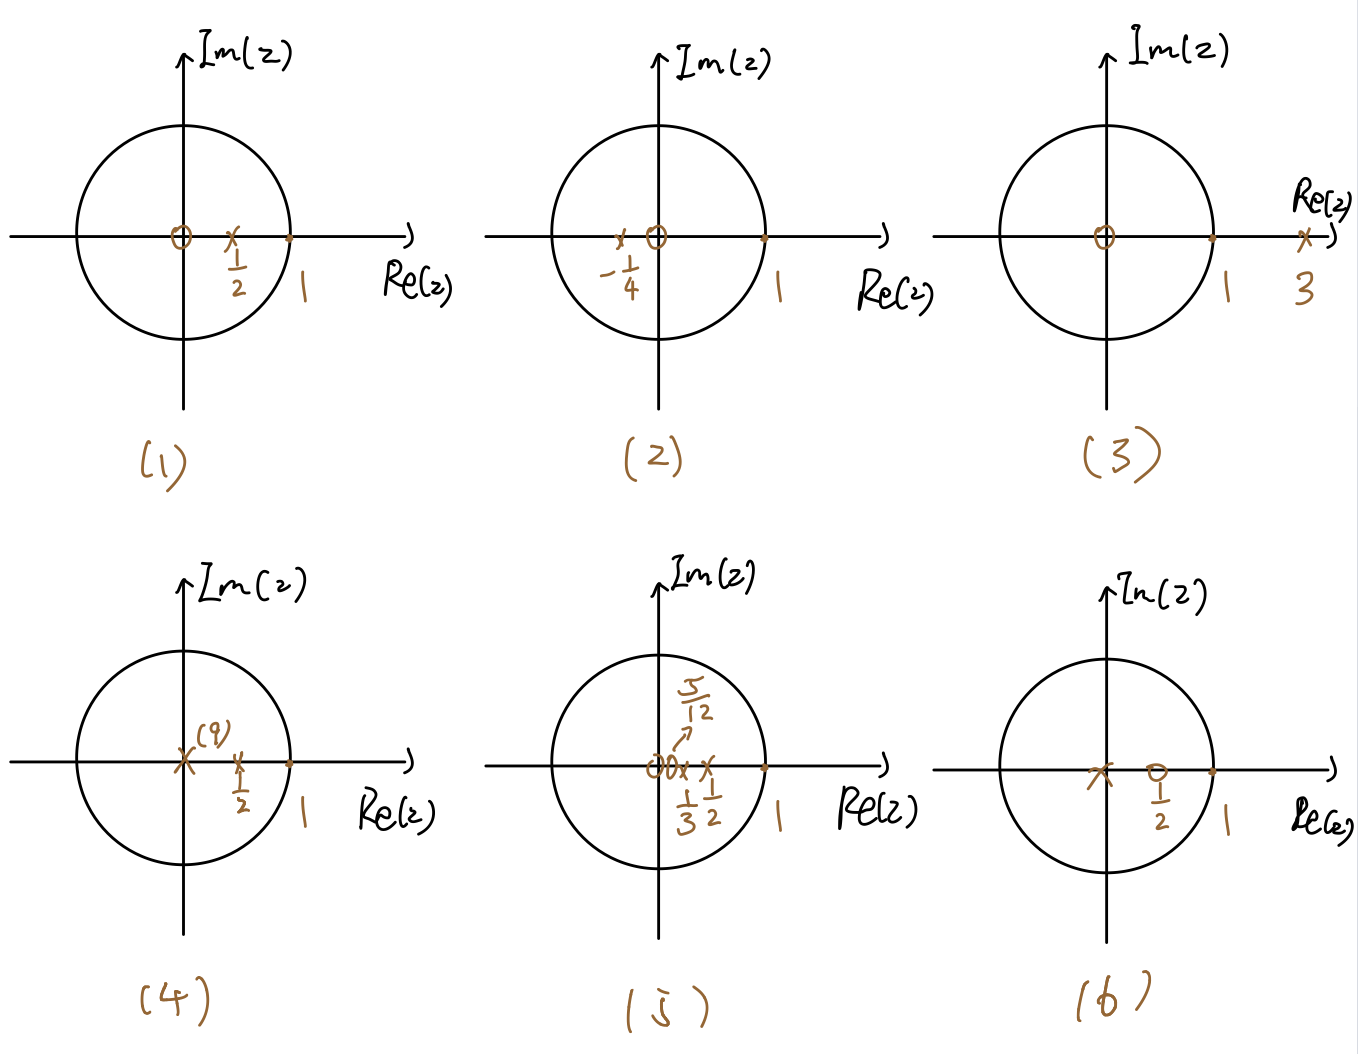
\includegraphics[width=0.9\linewidth]{pics/q10.png}
	\label{Figure:q10}
	\caption{q10-零极点图}
\end{figure}
% question_11
\question 求下列$X(z)$的逆变换$x[n]$。
\begin{enumerate}[(1)]
\item $X(z)=\frac{10}{(1-0.5z^{-1})(1-0.25z^{-1})},(|z|>0.5)$
\item $X(z)=\frac{10z^2}{(z-1)(z+1)},(|z|>1)$
\end{enumerate}
\begin{solution}
\begin{enumerate}[(1)]
	\item 由部分分式分解可得$X(z)=\frac{20}{1-0.5z^{-1}}-\frac{10}{1-0.25z^{-1}}$,从而$$x[n]=(20\cdot(\frac{1}{2})^n-10\cdot(\frac{1}{4})^n)u[n]$$
	\item 由部分分式分解易得$X(z)=\frac{5}{1-z^{-1}}+\frac{5}{1+z^{-1}}$,从而$$x[n]=5\cdot(1+(-1)^n)u[n]$$
\end{enumerate}
\end{solution}

% question_12
\question 求下列$X(z)$的逆变换$x[n]$。
\begin{enumerate}[(1)]
\item $X(z)=\frac{z^{-1}}{(1-6z^{-1})^2},(|z|>6)$
\item $X(z)=\frac{z^{-2}}{1+z^{-2}},(|z|>1)$
\end{enumerate}
\begin{solution}
\begin{enumerate}[(1)]
	\item 易得$X(z)=\frac{1}{6}\frac{6z^{-1}}{(1-6z^{-1})^2}$,所以$$x[n]=\frac{n}{6}6^nu[n]$$
	\item 易得$X(z)=1-\frac{1}{1+z^{-2}}=1-\frac{1-\cos\frac{\pi}{2}z^{-1}}{1-2z^{-1}\cos\frac{\pi}{2}+z^{-2}}$,所以$$x[n]=\delta[n]-\cos(\frac{\pi}{2}n)u[n]$$
\end{enumerate}
\end{solution}

% question_13
\question 用单边$z$变换解下列差分方程。
\begin{enumerate}[(1)]
\item $y[n+2]+y[n+1]+y[n]=u[n],y[0]=1,y[1]=2$
\item $y[n]+0.1y[n-1]-0.02y[n-2]=10u[n],y[-1]=4,y[-2]=6$
\item $y[n]=-5y[n-1]+nu[n],y[-1]=0$
\end{enumerate}
\begin{solution}
\begin{enumerate}[(1)]
	\item 对差分方程两边做z变换得到$$z^2(Y(z)-y[0]-y[1]z^{-1})+z(Y(z)-y[0])+Y(z)=\frac{1}{1-z^{-1}}$$从而$$\frac{Y(z)}{z}=\frac{\frac{1}{3}}{z-1}+\frac{-\frac{4}{\sqrt{3}}\sin(\frac{2\pi}{3})}{z^2+z+1}+\frac{\frac{2}{3}(z+\frac{1}{2})}{z^2+z+1}$$
	所以$$y[n]=[\frac{1}{3}-\frac{4}{\sqrt{3}}\sin(\frac{2n\pi}{3})+\frac{2}{3}\cos(\frac{2n\pi}{3})]u[n]$$
	\item 对差分方程两边做z变换得到$$Y(z)+0.1(z^{-1}Y(z)+4)-0.02(z^{-2}Y(z)+6+4z^{-1})=\frac{10}{1-z^{-1}}$$从而$$Y(z)=\frac{9.26}{1-z^{-1}}+\frac{0.66}{1+0.2z^{-1}}-\frac{0.2}{1-0.1z^{-1}}$$所以$$y[n]=(9.26+0.66(-0.2)^n-0.2(0.1)^n)u[n]$$
	\item 对差分方程两边做z变换得到$$Y(z)+5z^{-1}Y(z)=\frac{z^{-1}}{(1-z^{-1})^2}$$从而$$Y(z)=\frac{z^{2}}{(z-1)^2(z+5)}=\frac{\frac{1}{6}z^{-1}}{(1-z^{-1})^2}+\frac{\frac{5}{36}}{1-z^{-1}}-\frac{\frac{5}{36}}{1+5z^{-1}}$$所以$$y[n]=(\frac{n}{6}+\frac{5}{36}-\frac{5}{36}(-5)^n)u[n]$$
\end{enumerate}
\end{solution}

% question 14
\question (选做)你对这门课程的建议。
\begin{solution}
	在此作答。
\end{solution}


\end{questions}
\end{document}